% Demo lecture deck for the Co-learner README (original content, written for the demo).
\documentclass[aspectratio=169,11pt]{beamer}
\usepackage[sfdefault,scaled=.95]{FiraSans}
\usepackage{newtxsf}
\usepackage{tikz}
\usetikzlibrary{arrows.meta,calc,positioning,shapes.geometric}
\usepackage{booktabs}

\definecolor{ink}{HTML}{1F2430}
\definecolor{accent}{HTML}{3D5AFE}
\definecolor{accent2}{HTML}{E8590C}
\definecolor{soft}{HTML}{EEF1FF}
\definecolor{muted}{HTML}{6B7280}
\definecolor{good}{HTML}{2F9E44}

\setbeamertemplate{navigation symbols}{}
\setbeamercolor{normal text}{fg=ink,bg=white}
\setbeamercolor{structure}{fg=accent}
\setbeamercolor{frametitle}{fg=ink}
\setbeamercolor{block title}{fg=white,bg=accent}
\setbeamercolor{block body}{fg=ink,bg=soft}
\setbeamerfont{frametitle}{size=\Large,series=\bfseries}
\setbeamertemplate{itemize item}{\color{accent}\raisebox{.15ex}{\scalebox{.8}{$\blacktriangleright$}}}
\setbeamertemplate{itemize subitem}{\color{muted}--}
\setbeamertemplate{enumerate item}{\color{accent}\bfseries\insertenumlabel.}
\setbeamertemplate{blocks}[rounded][shadow=false]
\setbeamertemplate{frametitle}{%
  \vspace*{.55em}{\color{accent}\rule[-.12em]{.2em}{1.02em}}\hspace{.5em}%
  \insertframetitle\par\vspace*{-.1em}}
\setbeamertemplate{footline}{%
  \hbox to \paperwidth{\hspace*{1.1em}\color{muted}\scriptsize Computer Vision \,$\cdot$\, Lecture 3: Homographies and RANSAC\hfill\insertframenumber\hspace*{1.1em}}\vspace*{.7em}}
\setlength{\leftmargini}{1.4em}

\begin{document}

% 1 ---------------------------------------------------------------------------
{\setbeamertemplate{footline}{}
\begin{frame}
  \vspace*{2.2em}
  {\color{accent}\bfseries\small COMPUTER VISION \,$\cdot$\, LECTURE 3}\\[.9em]
  {\fontsize{30}{34}\selectfont\bfseries Homographies and RANSAC}\\[.7em]
  {\large\color{muted} Aligning photos into a panorama, even when some matches are wrong}\\[3.2em]
  
\begin{tikzpicture}
    \foreach \i/\c in {0/accent,1/accent2,2/good} \fill[\c] (\i*0.32,0) rectangle ++(.22,.22);
  \end{tikzpicture}\hspace{.6em}{\small\color{muted} A demo deck for the Co-learner README}
\end{frame}}

% 2 ---------------------------------------------------------------------------
\begin{frame}{From two photos to one panorama}
  \begin{columns}[T]
    \begin{column}{.47\textwidth}
      \begin{enumerate}\setlength{\itemsep}{.8em}
        \item \textbf{Match} features that appear in both photos.
        \item \textbf{Estimate} the transform that carries one photo onto the other.
        \item \textbf{Warp} the photo into the shared frame and \textbf{blend} the overlap.
      \end{enumerate}
      \vspace{1em}
      {\small\color{muted} This lecture: step 2, and how to survive the wrong matches from step 1.}
    \end{column}
    \begin{column}{.5\textwidth}
      \centering
      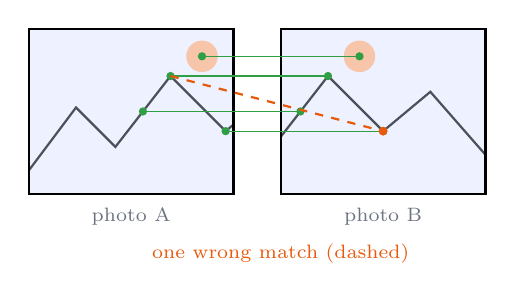
\begin{tikzpicture}[scale=1.0]
        % one scene (a skyline and a sun) seen by two photos: A shows world x in [0,2.6], B shows [1.2,3.8]
        \def\skyline{(0,0.3) -- (0.6,1.1) -- (1.1,0.6) -- (1.8,1.5) -- (2.5,0.8) -- (3.1,1.3) -- (3.8,0.5)}
        \begin{scope}
          \clip (0,0) rectangle (2.6,2.1);
          \fill[soft] (0,0) rectangle (2.6,2.1);
          \fill[accent2!35] (2.2,1.75) circle (.2);
          \draw[thick,ink!80] \skyline;
        \end{scope}
        \draw[thick] (0,0) rectangle (2.6,2.1);
        \begin{scope}[xshift=2.0cm]
          \begin{scope}
            \clip (1.2,0) rectangle (3.8,2.1);
            \fill[soft] (1.2,0) rectangle (3.8,2.1);
            \fill[accent2!35] (2.2,1.75) circle (.2);
            \draw[thick,ink!80] \skyline;
          \end{scope}
          \draw[thick] (1.2,0) rectangle (3.8,2.1);
        \end{scope}
        \node[muted,font=\scriptsize] at (1.3,-.28) {photo A};
        \node[muted,font=\scriptsize] at (4.5,-.28) {photo B};
        \foreach \x/\y in {1.8/1.5, 2.5/0.8, 2.2/1.75, 1.45/1.05} {
          \draw[good,thin] (\x,\y) -- (\x+2.0,\y);
          \fill[good] (\x,\y) circle (1.5pt); \fill[good] (\x+2.0,\y) circle (1.5pt);
        }
        \draw[accent2,thick,dashed] (1.8,1.5) -- (4.5,0.8);
        \fill[accent2] (4.5,0.8) circle (1.6pt);
        \node[accent2,font=\scriptsize] at (3.2,-.75) {one wrong match (dashed)};
      \end{tikzpicture}
    \end{column}
  \end{columns}
\end{frame}

% 3 ---------------------------------------------------------------------------
\begin{frame}{A homography maps a plane to a plane}
  In homogeneous coordinates a point $\mathbf{x}=(x,y,1)^\top$ in one image maps to
  \[
    \mathbf{x}' \;\sim\; H\,\mathbf{x},\qquad
    H=\begin{bmatrix} h_{11}&h_{12}&h_{13}\\ h_{21}&h_{22}&h_{23}\\ h_{31}&h_{32}&h_{33}\end{bmatrix}
  \]
  where $\sim$ means \emph{equal up to scale}: $H$ and $cH$ describe the same mapping.
  \vspace{.6em}
  \begin{itemize}\setlength{\itemsep}{.45em}
    \item 9 entries, 1 lost to scale: \textbf{8 degrees of freedom}.
    \item Exact when the scene is a plane, or when the camera only rotates about its center.
    \item Back to pixels: $x'=\dfrac{h_{11}x+h_{12}y+h_{13}}{h_{31}x+h_{32}y+h_{33}}$, \ $y'=\dfrac{h_{21}x+h_{22}y+h_{23}}{h_{31}x+h_{32}y+h_{33}}$.
  \end{itemize}
\end{frame}

% 4 ---------------------------------------------------------------------------
\begin{frame}{Each match gives two linear equations}
  Multiply out the division. With $\mathbf{h}=(h_{11},h_{12},h_{13},h_{21},h_{22},h_{23},h_{31},h_{32},h_{33})^\top$, one match $(x,y)\leftrightarrow(x',y')$ gives
  \[
    \begin{bmatrix}
      -x & -y & -1 & 0 & 0 & 0 & x x' & y x' & x'\\
      0 & 0 & 0 & -x & -y & -1 & x y' & y y' & y'
    \end{bmatrix}\mathbf{h}=\mathbf{0}.
  \]
  \begin{itemize}\setlength{\itemsep}{.45em}
    \item Linear in $\mathbf{h}$, even though the mapping itself is not.
    \item 8 unknowns (up to scale) and 2 equations per match: at least \textbf{4 matches}, no 3 of them on a line.
  \end{itemize}
\end{frame}

% 5 ---------------------------------------------------------------------------
\begin{frame}{The Direct Linear Transform (DLT)}
  \begin{columns}[T]
    \begin{column}{.56\textwidth}
      Stack the rows of all $n\ge 4$ matches into a $2n\times 9$ matrix $A$ and solve
      \[
        \min_{\mathbf{h}}\ \lVert A\mathbf{h}\rVert \quad\text{subject to}\quad \lVert\mathbf{h}\rVert=1 .
      \]
      With the SVD $A=U\Sigma V^\top$, the answer is the \textbf{last column of $V$}: the right singular vector with the smallest singular value.
    \end{column}
    \begin{column}{.4\textwidth}
      \begin{block}{Recipe}
        \small
        \begin{enumerate}\setlength{\itemsep}{.25em}
          \item build $A$ from the matches
          \item $U,\Sigma,V^\top=\mathrm{svd}(A)$
          \item $\mathbf{h}\leftarrow$ last row of $V^\top$
          \item reshape $\mathbf{h}$ to $3\times3$
        \end{enumerate}
      \end{block}
    \end{column}
  \end{columns}
  \vspace{.8em}
  {\small\color{muted} The constraint $\lVert\mathbf{h}\rVert=1$ rules out the useless answer $\mathbf{h}=\mathbf{0}$.}
\end{frame}

% 6 ---------------------------------------------------------------------------
\begin{frame}{Normalize the points before you solve}
  Pixel coordinates near $1000$ make the entries of $A$ range from $1$ to $xx'\approx 10^6$, so the SVD is badly conditioned.
  \vspace{.5em}
  \begin{block}{Normalized DLT}
    \begin{enumerate}\setlength{\itemsep}{.3em}
      \item Find $T$ (and $T'$) that move the points' centroid to the origin and scale them so their mean distance from it is $\sqrt{2}$.
      \item Run the DLT on $\hat{\mathbf{x}}=T\mathbf{x}$ and $\hat{\mathbf{x}}'=T'\mathbf{x}'$ to get $\hat H$.
      \item Undo the normalization: $H=T'^{-1}\,\hat H\,T$.
    \end{enumerate}
  \end{block}
  \vspace{.4em}
  {\small\color{muted} Same answer for perfect data; far more stable with noise.}
\end{frame}

% 7 ---------------------------------------------------------------------------
\begin{frame}{One wrong match ruins least squares}
  \begin{columns}[c]
    \begin{column}{.5\textwidth}
      \begin{itemize}\setlength{\itemsep}{.6em}
        \item Least squares weighs every match, so a single far-off point pulls the whole fit.
        \item Feature matching always produces some wrong matches (\emph{outliers}).
        \item We need a fit that \textbf{ignores} points it cannot explain.
      \end{itemize}
    \end{column}
    \begin{column}{.46\textwidth}
      \centering
      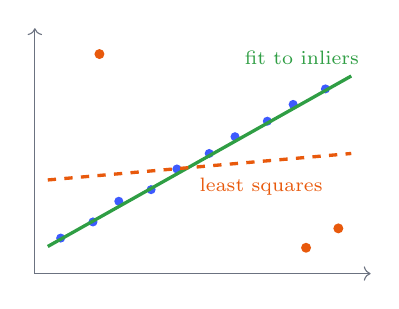
\begin{tikzpicture}[scale=.82]
        \draw[->,muted] (0,0) -- (5.2,0);
        \draw[->,muted] (0,0) -- (0,3.8);
        \foreach \x/\y in {0.4/0.55,0.9/0.8,1.3/1.12,1.8/1.3,2.2/1.62,2.7/1.86,3.1/2.12,3.6/2.36,4.0/2.62,4.5/2.86}
          \fill[accent] (\x,\y) circle (2pt);
        \foreach \x/\y in {1.0/3.4,4.2/0.4,4.7/0.7}
          \fill[accent2] (\x,\y) circle (2.2pt);
        \draw[very thick,good] (0.2,0.42) -- (4.9,3.06);
        \draw[very thick,accent2,dashed] (0.2,1.45) -- (4.9,1.86);
        \node[good,font=\scriptsize,anchor=west] at (3.1,3.35) {fit to inliers};
        \node[accent2,font=\scriptsize,anchor=west] at (2.4,1.35) {least squares};
      \end{tikzpicture}
    \end{column}
  \end{columns}
\end{frame}

% 8 ---------------------------------------------------------------------------
\begin{frame}{RANSAC: random sample consensus}
  \begin{columns}[T]
    \begin{column}{.55\textwidth}
      \begin{block}{Repeat $N$ times}
        \begin{enumerate}\setlength{\itemsep}{.35em}
          \item Pick \textbf{4 matches} at random.
          \item Fit $H$ to them with the DLT.
          \item Count the \textbf{inliers}: matches with $\lVert \mathbf{x}'_i - H(\mathbf{x}_i)\rVert < \varepsilon$ pixels.
        \end{enumerate}
      \end{block}
      \vspace{.3em}
      Keep the $H$ with the most inliers, then \textbf{refit} it on all of its inliers.
    \end{column}
    \begin{column}{.4\textwidth}
      \small
      \begin{itemize}\setlength{\itemsep}{.55em}
        \item $H(\mathbf{x})$: apply $H$, then divide by the third coordinate.
        \item $\varepsilon$ is a few pixels (for example 2 to 5).
        \item A sample of 4 inliers predicts the other inliers; a sample with an outlier usually predicts almost nothing.
      \end{itemize}
    \end{column}
  \end{columns}
\end{frame}

% 9 ---------------------------------------------------------------------------
\begin{frame}{How many samples are enough?}
  If a fraction $w$ of the matches are inliers, a sample of $s$ matches is all inliers with probability $w^s$.
  To succeed at least once with probability $p$:
  \[
    N=\left\lceil\frac{\log(1-p)}{\log\left(1-w^{s}\right)}\right\rceil
  \]
  \vspace{-.3em}
  \begin{columns}[c]
    \begin{column}{.45\textwidth}
      \centering
      \begin{tabular}{@{}ccc@{}}
        \toprule
        inlier fraction $w$ & $s$ & $N$ \;($p=0.99$)\\
        \midrule
        0.9 & 4 & 5\\
        0.7 & 4 & 17\\
        0.5 & 4 & 72\\
        0.3 & 4 & 567\\
        \bottomrule
      \end{tabular}
    \end{column}
    \begin{column}{.47\textwidth}
      \small
      \begin{itemize}\setlength{\itemsep}{.5em}
        \item $N$ depends on $w$ and $s$, not on how many matches there are.
        \item Fewer points per sample help: that is why we use the minimal 4.
      \end{itemize}
    \end{column}
  \end{columns}
\end{frame}

% 10 --------------------------------------------------------------------------
\begin{frame}{Warp, then blend}
  \begin{columns}[T]
    \begin{column}{.52\textwidth}
      \textbf{Backward warping.} For every pixel $\mathbf{p}$ of the output canvas, look up the source image at $H^{-1}\mathbf{p}$ and interpolate (bilinear). Every output pixel gets a value; no holes.
      \vspace{.8em}

      \textbf{Feathering.} Weight each image by its pixel's distance to that image's border (a distance transform), then average:
      \[
        I(\mathbf{p})=\frac{\sum_k w_k(\mathbf{p})\,I_k(\mathbf{p})}{\sum_k w_k(\mathbf{p})}
      \]
    \end{column}
    \begin{column}{.44\textwidth}
      \centering
      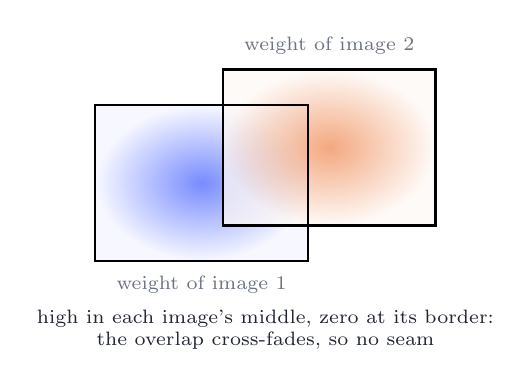
\begin{tikzpicture}[scale=.9]
        \shade[inner color=accent!70,outer color=accent!4] (0,0) rectangle (3.0,2.2);
        \shade[inner color=accent2!70,outer color=accent2!4,opacity=.75] (1.8,0.5) rectangle (4.8,2.7);
        \draw[thick] (0,0) rectangle (3.0,2.2);
        \draw[thick] (1.8,0.5) rectangle (4.8,2.7);
        \node[font=\scriptsize,muted,anchor=north] at (1.5,-.08) {weight of image 1};
        \node[font=\scriptsize,muted,anchor=south] at (3.3,2.78) {weight of image 2};
        \node[font=\scriptsize,ink,align=center,anchor=north] at (2.4,-.55) {high in each image's middle, zero at its border:\\the overlap cross-fades, so no seam};
      \end{tikzpicture}
    \end{column}
  \end{columns}
\end{frame}

% 11 --------------------------------------------------------------------------
\begin{frame}{Summary}
  \begin{itemize}\setlength{\itemsep}{.8em}
    \item A homography $H$ (8 degrees of freedom) maps one view of a plane, or of a rotating camera, onto another.
    \item The DLT turns 4 or more matches into $A\mathbf{h}=\mathbf{0}$; the SVD gives $\mathbf{h}$. Normalize first.
    \item RANSAC fits $H$ to random minimal samples and keeps the one most matches agree with.
    \item Backward warping fills the canvas; distance-weighted blending hides the seams.
  \end{itemize}
  \vspace{1.2em}
  {\small\color{muted} Next lecture: stereo and depth.}
\end{frame}

\end{document}
